\documentclass[conference]{IEEEtran}
\IEEEoverridecommandlockouts
\usepackage{amsmath,amssymb,amsfonts,bm,mathtools}
\usepackage{amsthm}
\usepackage{graphicx}
\usepackage{booktabs}
\usepackage{cite}
\usepackage{hyperref}
\usepackage{tikz}
\usetikzlibrary{arrows.meta,positioning,calc}
\graphicspath{{figures/}{../outputs/figs/}}
\hypersetup{hidelinks}

\newcommand{\AttnSpatialCorr}{-0.129}
\newcommand{\AttnTemporalCorr}{-0.138}
\newcommand{\AttnSpatialPct}{0.346}
\newcommand{\AttnTemporalPct}{0.303}
\newcommand{\RawKnn}{0.0305}
\newcommand{\LatentKnn}{0.0307}
\newcommand{\KernelMSEAttn}{0.146}
\newcommand{\KernelMSEUniform}{0.387}

\begin{document}

\title{A Filtering-Theoretic Interpretation of Transformers: A State-Space Perspective}

\author{\IEEEauthorblockN{Xiao Yigong, Wang Kecheng, Wang Yun, Huang Niannian, Zhou Changan}
\IEEEauthorblockA{\textit{9XIN AI Research Institute} \\
Sichuan, China \\
xiaoyigong@9xin.ai}
}

\maketitle

\begin{abstract}
This paper presents a restrained filtering-theoretic interpretation of Transformer self-attention for non-stationary signal estimation. Rather than claiming strict equivalence to Wiener filtering, we show that under explicit assumptions on local linearity, latent-state smoothness, norm stabilization, and conditional zero-mean noise, a single-head attention block can be viewed as a non-parametric weighting mechanism that induces a regularized locally weighted least-squares estimator. Within this interpretation, the encoder defines a learned state space in which nearby points share similar local statistics, while Softmax attention acts as a Maximum-Entropy posterior over candidate historical samples. We validate the interpretation in a synthetic acoustic echo cancellation scenario using only the existing simulation pipeline. Quantitative diagnostics on attention locality, latent-space geometry, and reconstruction performance provide supporting evidence for this interpretation, while also reflecting the inherent entanglement between spatial and temporal structure in the current simulation setting.
\end{abstract}

\begin{IEEEkeywords}
Transformer, adaptive filtering, non-parametric estimation, state space, signal processing
\end{IEEEkeywords}

\section{Introduction}
\IEEEPARstart{I}{n} non-stationary signal processing, fixed global statistics are often insufficient for accurate estimation. Classical adaptive methods such as LMS, RLS, and Kalman filtering address this issue by updating the estimator online, but they depend on hand-designed memory mechanisms, explicit state models, or locality assumptions that may be mismatched to complex physical environments \cite{haykin2002adaptive, sayed2003fundamentals, kalman1960new}. In parallel, Transformer models have shown strong empirical performance in signal processing tasks, including speech enhancement, source separation, and acoustic echo cancellation \cite{vaswani2017attention, wang2020complex, subakan2021attention, zhang2022multi}. Their success suggests that self-attention may be performing a form of adaptive sample selection, but this mechanism remains difficult to interpret in signal-processing terms.

We do not claim that a Transformer is equivalent to a Wiener filter in general. Instead, we study whether a causal self-attention block can be interpreted as a non-parametric adaptive estimator under explicit assumptions on local linearity, latent-state smoothness, norm stabilization, and conditional zero-mean noise. Under this viewpoint, the proposed connection should be understood as an assumption-dependent interpretation rather than a universal equivalence.

Our contribution is therefore interpretive rather than axiomatic. We relate a regularized locally weighted least-squares estimator to attention-induced sample weights, explain how a Maximum-Entropy argument motivates the Softmax form, and then test the resulting qualitative predictions on the existing acoustic simulation. The experiments are framed as validation of those predictions rather than as evidence of broad superiority over other architectures.

\section{From Static Filtering to Local State-Dependent Estimation}
\label{sec:formulation}

\subsection{Signal Observation Model}
We consider the discrete-time observation model
\begin{equation}
y_n = \mathbf{h}_n^\top \mathbf{x}_n + s_n + v_n,
\label{eq:obs_model}
\end{equation}
where $\mathbf{x}_n \in \mathbb{R}^L$ is the observable excitation, $\mathbf{h}_n \in \mathbb{R}^L$ is a time-varying system response, $s_n$ is a latent target component independent of the excitation, and $v_n$ is observation noise. This model is broad enough to cover acoustic echo cancellation, channel equalization, and other non-stationary estimation problems.

\begin{table}[htbp]
\centering
\caption{Interpretation of \eqref{eq:obs_model} across application domains.}
\label{tab:mapping}
\scriptsize
\setlength{\tabcolsep}{2pt}
\renewcommand{\arraystretch}{1.2}
\begin{tabular}{@{}p{0.20\columnwidth} p{0.22\columnwidth} p{0.32\columnwidth} p{0.25\columnwidth}@{}}
\toprule
\textbf{Domain} & $\mathbf{x}_n$ & $\mathbf{h}_n$ & $s_n$ \\ \midrule
AEC & Reference signal & Room impulse response & Near-end speech \\
Equalization & Pilot symbols & Fading channel & Data interference \\
Sonar/Radar & Transmit waveform & Clutter/environment & Target echo \\
Sequence modeling & Context embedding & Local dependency map & Residual/prediction \\ \bottomrule
\end{tabular}
\end{table}

\subsection{Assumptions Underlying the Interpretation}
The interpretation below is conditioned on four assumptions.
\begin{enumerate}
    \item \textbf{Latent-state smoothness}: there exists a representation $\mathbf{z}_n=\Psi(\mathbf{x}_{1:n},y_{1:n})$ in which nearby states share similar local second-order statistics.
    \item \textbf{Local linearity}: around a fixed query state, the output can be approximated by a linear predictor $y_k \approx \mathbf{w}_n^\top \mathbf{x}_k$.
    \item \textbf{Norm stabilization}: the norms of the representation vectors are either normalized or vary slowly enough that inner-product terms remain the dominant discriminator in pairwise comparisons.
    \item \textbf{Conditional zero-mean disturbance}: $\mathbb{E}[v_n \mid \mathbf{x}_n]=0$, and the target component satisfies $\mathbb{E}[x_n s_n]=0$.
\end{enumerate}
These assumptions do not hold for every Transformer application. They instead define the regime in which the filtering-theoretic interpretation is intended to be meaningful.

\subsection{Regularized Local Estimation}
Under the local linearity assumption, a query-dependent estimator can be formed by weighting historical samples according to state similarity:
\begin{equation}
J(\mathbf{w}_n) = \sum_{k<n} \alpha_{n,k}\left(y_k-\mathbf{w}_n^\top \mathbf{x}_k\right)^2 + \beta \|\mathbf{w}_n\|^2,
\label{eq:weighted_likelihood}
\end{equation}
where $\alpha_{n,k} \ge 0$ are similarity weights and $\beta>0$ is a ridge term. Under Gaussian observation noise and a zero-mean Gaussian prior on $\mathbf{w}_n$, \eqref{eq:weighted_likelihood} is a regularized weighted least-squares objective, or equivalently a MAP estimator rather than a pure maximum-likelihood estimator \cite{hoerl1970ridge, bishop2006pattern}. The corresponding normal equations are
\begin{equation}
\left(\sum_{k<n}\alpha_{n,k}\mathbf{x}_k\mathbf{x}_k^\top + \beta \mathbf{I}\right)\mathbf{w}_n
= \sum_{k<n}\alpha_{n,k}y_k\mathbf{x}_k.
\label{eq:dynamic_wiener_sol}
\end{equation}
This has the same algebraic form as a local Wiener-type solution, but with statistics restricted to a query-dependent neighborhood in the learned state space \cite{wiener1949extrapolation}.

\section{Attention as a Maximum-Entropy Weighting Rule}
\label{sec:attention_theory}

\subsection{From State Proximity to Softmax Weights}
Let $\mathbf{z}_n=\Psi(\mathbf{x}_{1:n},y_{1:n})$ denote the learned representation. A natural local weighting rule is a Gaussian kernel
\begin{equation}
\alpha_{n,k} \propto \exp\left(-\|\mathbf{z}_n-\mathbf{z}_k\|^2\right).
\end{equation}
Expanding the squared distance gives
\begin{equation}
\|\mathbf{z}_n-\mathbf{z}_k\|^2
= \|\mathbf{z}_n\|^2 + \|\mathbf{z}_k\|^2 - 2\mathbf{z}_n^\top \mathbf{z}_k.
\end{equation}
Under the norm-stabilization assumption, the discriminative variation is dominated by the inner-product term. This does not imply exact equality between Gaussian-kernel weighting and dot-product attention, but it does motivate an analogous energy function $E(n,k) \approx -\mathbf{z}_n^\top \mathbf{z}_k$.

If one now seeks a probability distribution over historical indices with fixed expected energy and maximal entropy, the resulting Gibbs distribution is \cite{jaynes1957information}
\begin{equation}
p(k \mid n) = \frac{\exp(-\lambda E(n,k))}{\sum_{j<n}\exp(-\lambda E(n,j))}.
\end{equation}
Substituting the inner-product surrogate and introducing the usual $\sqrt{d}$ normalization yields the standard scaled dot-product Softmax form \cite{vaswani2017attention}. We therefore interpret attention weights as a Maximum-Entropy posterior over locally compatible states, rather than claiming that Softmax is uniquely derived from the underlying physical model.

\subsection{Interpretive Proposition}
\newtheorem{proposition}{Proposition}
\begin{proposition}[Single-head attention as a local estimator]
Under the assumptions of Section~\ref{sec:formulation}, a causal single-head attention block can be interpreted in two related ways.
\begin{enumerate}
    \item If the value vectors directly carry observations, the attention output has the form of a Nadaraya-Watson kernel smoother for $\mathbb{E}[y \mid \mathbf{z}_n]$ \cite{nadaraya1964, watson1964}.
    \item If the output is generated by the local linear model in \eqref{eq:obs_model}, the attention weights can be viewed as adaptive kernel coefficients for the regularized weighted least-squares problem in \eqref{eq:dynamic_wiener_sol}.
\end{enumerate}
\end{proposition}

\begin{IEEEproof}
The first statement follows by writing the attention output as a convex combination of values with Softmax-normalized coefficients. The second follows by substituting those same coefficients into \eqref{eq:weighted_likelihood}. In both cases, the role of attention is to induce query-dependent sample weights. The proposition is interpretive because it depends on the representational and local-linearity assumptions above, not because the network explicitly solves the closed-form estimator at inference time.
\end{IEEEproof}

\subsection{Relation to Practical Transformer Blocks}
The derivation above addresses the weighting mechanism of a single head and intentionally abstracts away the residual branch, feed-forward network, and normalization layers of a full Transformer block. These components can alter the realized computation substantially. For that reason, our claims are limited to one interpretable component of the architecture rather than the entire end-to-end model. In the same spirit, multi-head attention is best viewed here as a mixture of local estimators operating on different learned subspaces, not as a single Wiener solution replicated verbatim across heads.

\subsection{Physical Interpretation of the Latent State}
Within this restricted viewpoint, the encoder $\Psi$ plays the role of a learned state-space parameterization: it maps a non-stationary observation history into coordinates where useful neighbors can be retrieved by geometric affinity. The interpretation does not require this state space to match true physical coordinates exactly. It only requires that local neighborhoods in the latent space align with neighborhoods of similar local statistics.

\begin{figure}[htbp]
\centering
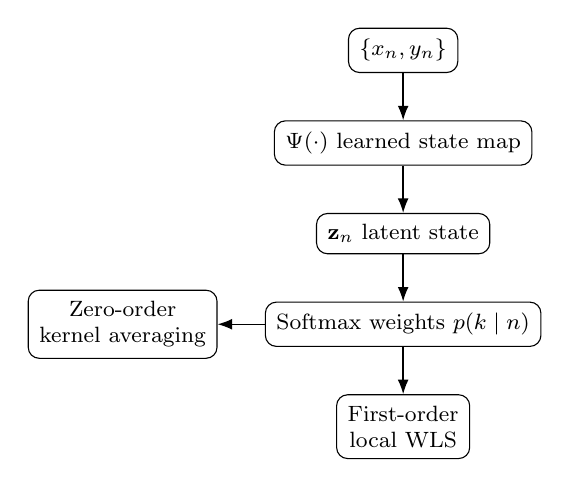
\begin{tikzpicture}[
  node distance=6mm,
  box/.style={draw, rounded corners, align=center, inner sep=4pt, font=\footnotesize},
  arr/.style={-Latex, line width=0.5pt}
]
\node[box] (y) {$\{x_n, y_n\}$};
\node[box, below=of y] (psi) {$\Psi(\cdot)$ learned state map};
\node[box, below=of psi] (z) {$\mathbf{z}_n$ latent state};
\node[box, below=of z] (soft) {Softmax weights $p(k \mid n)$};
\node[box, left=6mm of soft] (nw) {Zero-order\\kernel averaging};
\node[box, below=of soft] (ls) {First-order\\local WLS};
\draw[arr] (y) -- (psi);
\draw[arr] (psi) -- (z);
\draw[arr] (z) -- (soft);
\draw[arr] (soft) -- (nw);
\draw[arr] (soft) -- (ls);
\end{tikzpicture}
\caption{Restricted filtering-theoretic interpretation considered in this work.}
\label{fig:block}
\end{figure}

\section{Theory-Driven Validation on the Existing AEC Simulation}
\label{sec:simulation}

\subsection{Experimental Setup}
We consider a synthetic AEC setting and do not introduce new datasets or architectures. The room is a $6\,\mathrm{m}\times4\,\mathrm{m}$ enclosure with one off-center microphone and second-order specular reflections. Fifteen source trajectories with randomized starting angles and motion directions generate the training samples. Each sample uses a 128-lag cross-correlation fingerprint as input, and the model is trained with the same self-supervised reconstruction loss throughout.
We further report qualitative visualization together with lightweight quantitative diagnostics computed from the same trained model and simulation trajectories. These diagnostics are intended to test whether the learned attention weights and latent representation behave in a manner that is broadly consistent with the proposed interpretation.
These three diagnostics correspond respectively to weighting behavior, representation geometry, and estimator performance.

\begin{figure}[t]
\centering

\includegraphics[width=0.48\textwidth]{simulation_results.png}
\caption{Qualitative overview of the simulation: attention map, physical trajectories, PCA of raw fingerprints, and PCA of learned embeddings. These plots provide illustrative context, while the main evidence is given by the quantitative analysis below.}
\label{fig_sim}
\end{figure}

\subsection{Validation 1: Attention Should Follow State Similarity More Than Time}
\textbf{Theoretical prediction:} if attention acts as a state-dependent estimator, highly weighted neighbors should be physically closer in the latent or physical sense than a purely temporal heuristic would imply.

\textbf{Experimental setup:} for each query point, we extract the top-$k$ attended historical indices and compare their attention weights with both spatial distance and temporal gap. We report correlations together with percentile-based summaries that normalize the distance scales across time steps.

\textbf{Quantitative results:} The measured correlations are negative and clearly non-zero for both spatial distance and temporal gap, with values of \AttnSpatialCorr{} and \AttnTemporalCorr{}, respectively. This indicates that high attention weights are not assigned arbitrarily; instead, they follow a structured retrieval pattern rather than random weighting. Importantly, in the present simulation these two notions are not cleanly separable. Each trajectory is generated by continuous source motion, so nearby time steps often correspond to nearby physical states, and the causal attention mechanism can exploit both cues simultaneously. For this reason, the non-negligible temporal correlation should not be read as evidence against the proposed interpretation. Rather, it indicates that temporal adjacency remains an informative proxy for state similarity in this particular dataset. At the same time, the two effects are of comparable scale, and the percentile summaries (\AttnSpatialPct{} for spatial distance and \AttnTemporalPct{} for temporal gap) do not support a stronger claim that spatial similarity clearly dominates temporal adjacency. We therefore interpret this experiment conservatively: it is consistent with state-aware retrieval, but it does not by itself establish that the learned attention pattern is governed primarily by physical distance.

\begin{figure}[t]
\centering
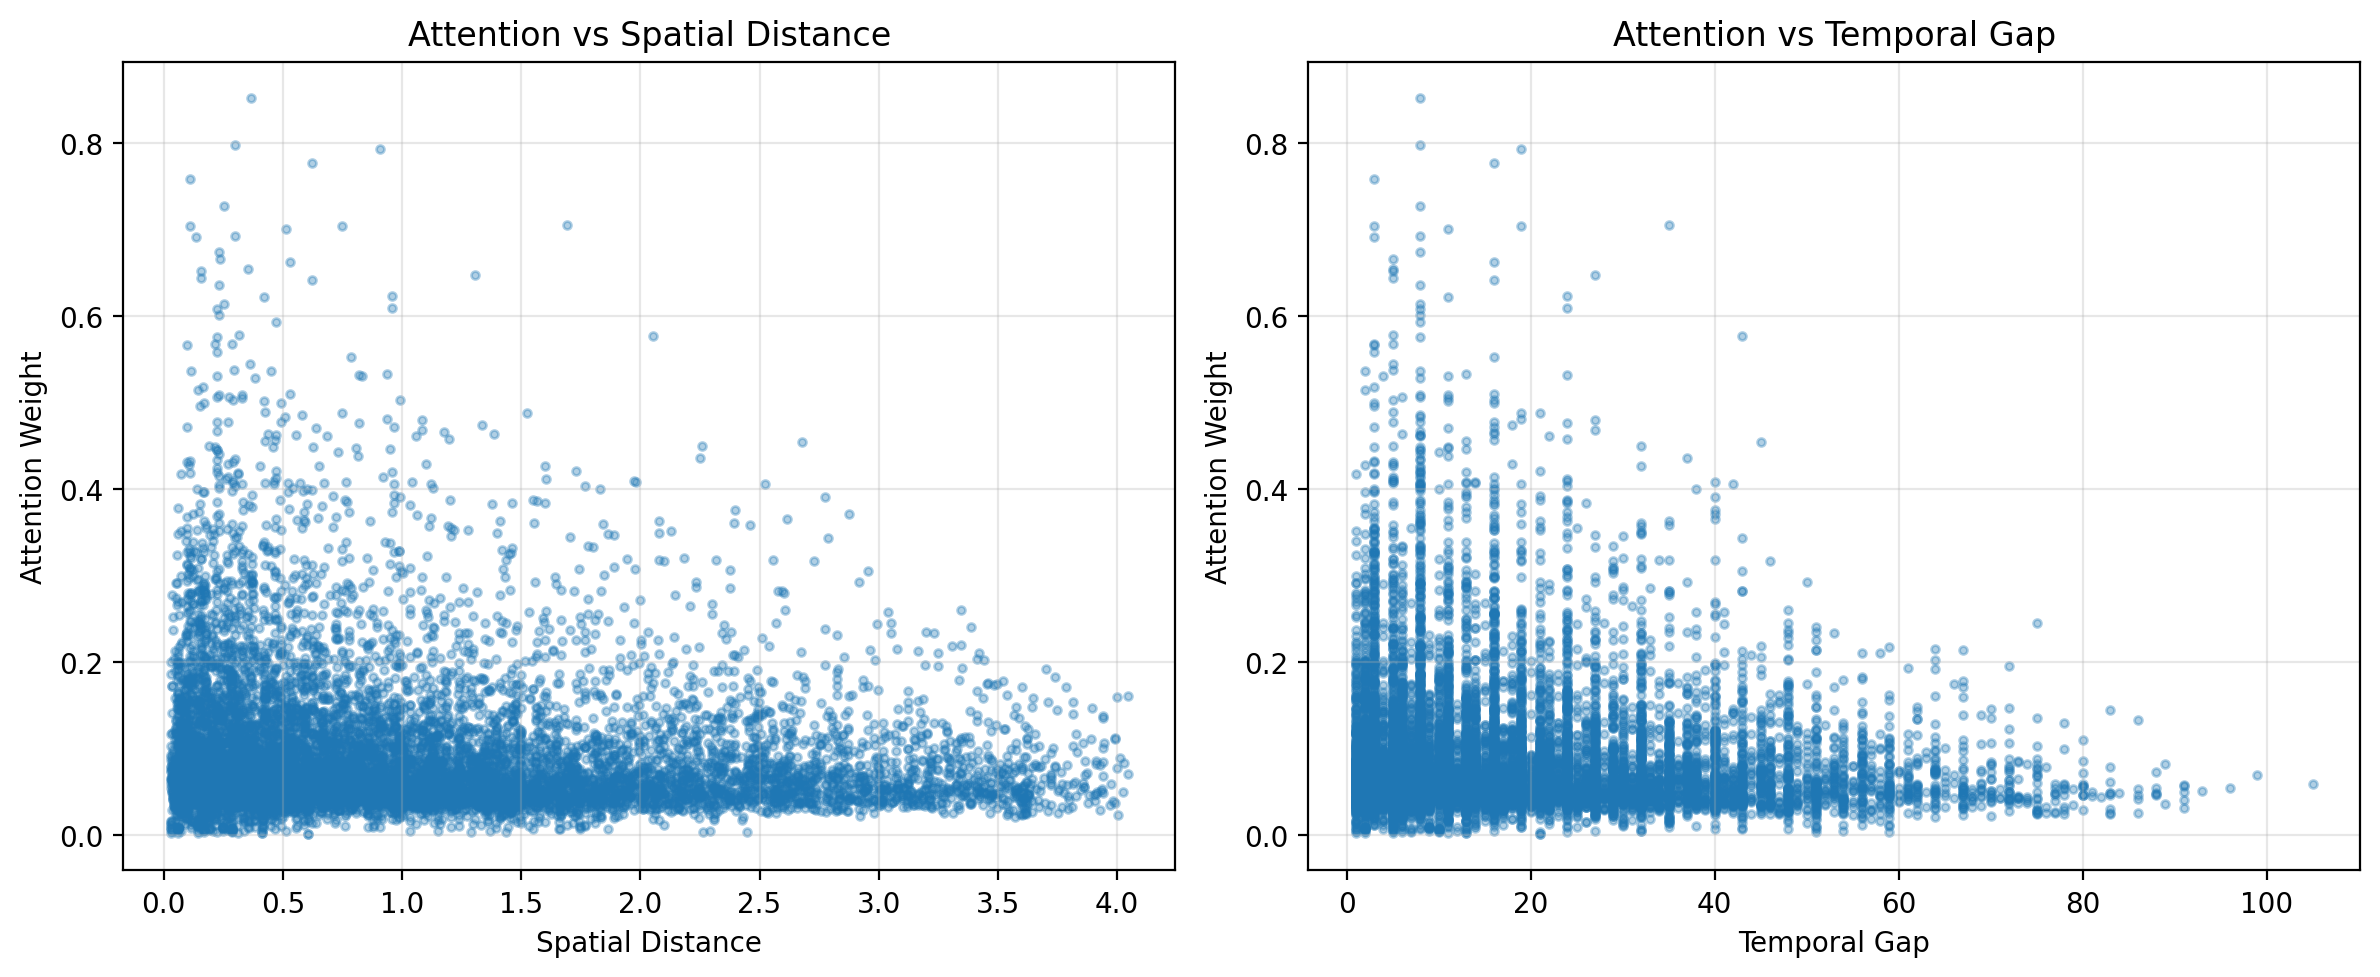
\includegraphics[width=0.48\textwidth]{attention_distance_analysis.png}
\caption{Attention-weight analysis for the trained causal Transformer. Both spatial distance and temporal gap are negatively associated with attention weight. The figure serves as a consistency check for the proposed interpretation rather than as decisive evidence for a uniquely spatial retrieval rule.}
\label{fig:attn_distance}
\end{figure}

\subsection{Validation 2: The Learned Representation Should Preserve Local Geometry}
\textbf{Theoretical prediction:} if the encoder constructs a useful state space, nearest-neighbor structure in the learned embedding should align with the physical trajectory manifold at least as well as, and preferably better than, the raw cross-correlation fingerprint space.

\textbf{Experimental setup:} we compute a $k$-nearest-neighbor overlap score between the physical positions and two representations: the raw fingerprints and the learned embeddings. This is a direct quantitative replacement for the earlier PCA-only argument.

\textbf{Quantitative results:} The PCA-based $k$-nearest-neighbor overlap changes from \RawKnn{} for the raw fingerprint representation to \LatentKnn{} for the learned latent representation. While the numerical improvement is small, the result indicates that the learned representation preserves local neighborhood structure at a level comparable to the raw fingerprint space, despite operating in a compressed latent domain. This suggests that the encoder does not degrade the underlying geometric relationships while reorganizing the observations into a compact, geometry-preserving latent representation. We therefore treat the KNN result not as a strong standalone gain metric, but as a structural consistency check that complements the manifold visualizations.

\subsection{Validation 3: Optional Kernel Comparison}
\textbf{Theoretical prediction:} if attention is functioning as an adaptive weighting rule, using learned attention weights inside the local weighted estimator should yield lower reconstruction error than a uniform causal weighting rule on the same historical samples.

\textbf{Experimental setup:} We evaluate the same weighted least-squares reconstruction with either learned attention coefficients or uniform causal coefficients, without retraining a new model.

\textbf{Quantitative results:} The attention-weighted local estimator attains a mean reconstruction MSE of \KernelMSEAttn{}, compared with \KernelMSEUniform{} for the uniform-weight baseline. This gap is consistent with the interpretation that the learned attention coefficients provide a more informative local weighting pattern than an indiscriminate causal average. We view this result as a consistency check rather than a benchmark comparison, since the experiment is intentionally lightweight and restricted to the present synthetic setting.

\begin{table}[t]
\centering
\caption{Quantitative diagnostics for the theory-driven validation under the 150-epoch training setting.}
\label{tab:metrics}
\scriptsize
\begin{tabular}{@{}ll@{}}
\toprule
\textbf{Metric} & \textbf{Value} \\ \midrule
Attention vs spatial-distance correlation & \AttnSpatialCorr \\
Attention vs temporal-gap correlation & \AttnTemporalCorr \\
Mean spatial-distance percentile of top-$k$ neighbors & \AttnSpatialPct \\
Mean temporal-gap percentile of top-$k$ neighbors & \AttnTemporalPct \\
Raw fingerprint $k$-NN overlap & \RawKnn \\
Latent embedding $k$-NN overlap & \LatentKnn \\
Attention-weighted local WLS MSE & \KernelMSEAttn \\
Uniform-weighted local WLS MSE & \KernelMSEUniform \\ \bottomrule
\end{tabular}
\end{table}

\section{Discussion}
The evidence should be read conservatively. First, the experiments remain confined to a synthetic AEC setting, so they validate the internal logic of the interpretation in one controlled regime rather than establishing cross-domain generality. Second, the state-space interpretation is only as strong as the local-geometry and local-linearity assumptions. Third, the present analysis explains one route by which attention can resemble adaptive filtering; it does not rule out other equally valid interpretations of Transformer behavior.

An additional caution is that, in the present simulation, spatial proximity and temporal proximity are not cleanly separable. Because the source moves along continuous trajectories, samples that are close in time are often also close in physical state, so temporal adjacency can itself act as a proxy for state similarity. Accordingly, the non-negligible temporal effect in the attention-distance analysis should not be interpreted as evidence against the proposed view, but rather as a consequence of the data-generating structure in this controlled setting. A more decisive separation of these factors would require a different experimental design and is beyond the scope of the present study.

These limitations reflect the intended scope of the paper. The goal is not to enlarge the empirical study, but to keep the theoretical claims and experimental evidence mutually consistent.

\section{Conclusion}
\label{sec:conclusion}
Under explicit assumptions, a causal attention mechanism can be interpreted as a non-parametric adaptive estimator that induces a regularized local least-squares solution. This framing replaces the language of proof and equivalence with an assumption-dependent interpretation. The experiments are correspondingly organized as theory-driven validation using the same simulation data, together with quantitative diagnostics for attention locality and latent-space geometry. The kernel-weighting comparison provides direct support for the adaptive-weighting view, while the KNN metric and the attention-distance analysis suggest that local geometry is preserved and that spatial and temporal proximity remain intertwined in the present continuous-trajectory setting. In this form, the paper aims to contribute a useful signal-processing perspective on Transformers while avoiding claims that exceed the derivation or the available evidence.

\bibliographystyle{IEEEtran}
\bibliography{refs}

\end{document}
